%
% File arr.tex
%
%% Based on the style files for ACL-IJCNLP 2021, which were % Based on the style
%files for EMNLP 2020, which were % Based on the style files for ACL 2020, which
%were % Based on the style files for ACL 2018, NAACL 2018/19, which were % Based
%on the style files for ACL-2015, with some improvements %  taken from the
%NAACL-2016 style % Based on the style files for ACL-2014, which were, in turn,
%% based on ACL-2013, ACL-2012, ACL-2011, ACL-2010, ACL-IJCNLP-2009, %
%EACL-2009, IJCNLP-2008... % Based on the style files for EACL 2006 by
%%e.agirre@ehu.es or Sergi.Balari@uab.es % and that of ACL 08 by Joakim Nivre
%and Noah Smith

\documentclass[11pt,a4paper]{article}
\usepackage[hyperref]{arr}
\usepackage{times}
\usepackage{latexsym}
\usepackage{amsmath}
\usepackage{graphicx}
\renewcommand{\UrlFont}{\ttfamily\small}
\newcommand{\wvect}[1]{\accentset{\rightharpoonup}{#1}}

\makeatletter
\def\blfootnote{\gdef\@thefnmark{}\@footnotetext}
\makeatother

% This is not strictly necessary, and may be commented out, but it will improve
% the layout of the manuscript, and will typically save some space.
\usepackage{microtype}

\aclfinalcopy % Uncomment this line for the final submission
%\def\aclpaperid{***} %  Enter the acl Paper ID here

%\setlength\titlebox{5cm} You can expand the titlebox if you need extra space to
% show all the authors. Please do not make the titlebox smaller than 5cm (the
% original size); we will check this in the camera-ready version and ask you to
% change it back.

% For proper rendering and hyphenation of words containing Latin characters
% (including in bib files)
\usepackage[T1]{fontenc}
% For Vietnamese characters \usepackage[T5]{fontenc} See
% https://www.latex-project.org/help/documentation/encguide.pdf for other
% character sets

% This assumes your files are encoded as UTF8
\usepackage[utf8]{inputenc}

\title{Learned Gender Bias in Wikipedia Persists with Time,\\ as measured by WEAT Scores }

\author{Blake Vente \\
  Hunter College\\
  \texttt{Ralph.Vente09@myhunter.cuny.edu}}

\date{\today{}}

\begin{document}
\maketitle
\begin{abstract}
  Word embeddings exhibit desirable properties when converting natural language
  to numerical vector representations. However, embeddings often internalize
  associations that parrot stereotypes pertaining to  race, gender, and culture.
  Researchers have attempted to mitigate word embedding bias by altering the
  model after training, or changing the loss function, but to address bias
  comprehensively, \citet{origins-1810-03611} turn to the data where these
  biases originate. This work examines the differences in word embedding
  representations learned of Wikipedia a decade apart, finding minimal
  differences between them. This work finds that larger window sizes correlate
  with higher WEAT scores and higher performance on analogy and similarity
  datasets.
\end{abstract}

\section{Introduction}

Distributional semantic models represent words with fixed-dimensional vectors
based on the how words are used in context of other words in large quantities of
unstructured text \cite{lison2017redefining}. Word embedding models in
particular, represent words as low-dimensional vectors intended to capture
functional and topical relations between words \cite{lison2017redefining}.
\blfootnote{My source code associated with this paper is located at \href{https://github.com/rvente/word-embedding-bias}{rvente/word-embedding-bias} on GitHub.}
\subsection{Density of Word Representations}

Classical approaches would represent words using one-hot encoding, with
higher-dimensional vectors and binary elements. The one-hot representation of
puppy would be a 1 in the `puppy' dimension and zeros in all other components.
Since vocabulary size is large even for moderately-sized corpora and since the
dimensions of the vector depends on the vocabulary size, one-hot representations
constrain the complexity of machine learning models where training complexity
depends on the number of dimensions in the input. By contrast, word embeddings
are fixed-dimensional representations with fixed dimension size of around 300
compared to the vocabularies of at least tens of thousands of words.

Word embeddings have a wide variety of applications for natural language
processing tasks including part-of-speech tagging, syntactic parsing, and named
entity recognition \cite{lison2017redefining}. In general, word embeddings are
broadly applicable for any machine learning system that operates on vectors,
including deep learning models and . Independently of their training mechanisms,
word embeddings reproduce the bias intrinsic to the data they were trained on.

\begin{figure}
  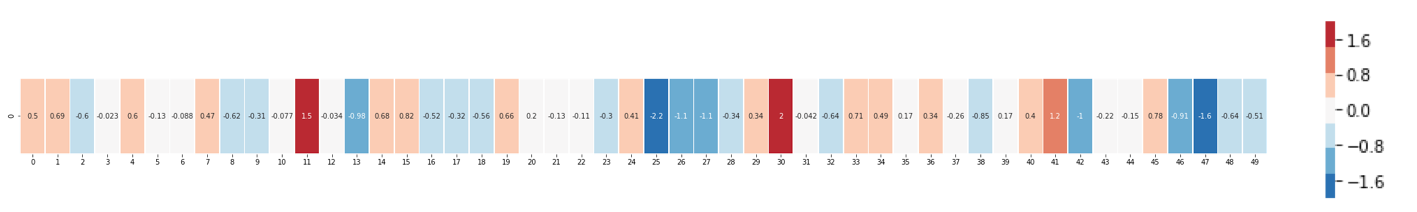
\includegraphics[width=.5\textwidth]{figures/king-colored-embedding.png}
  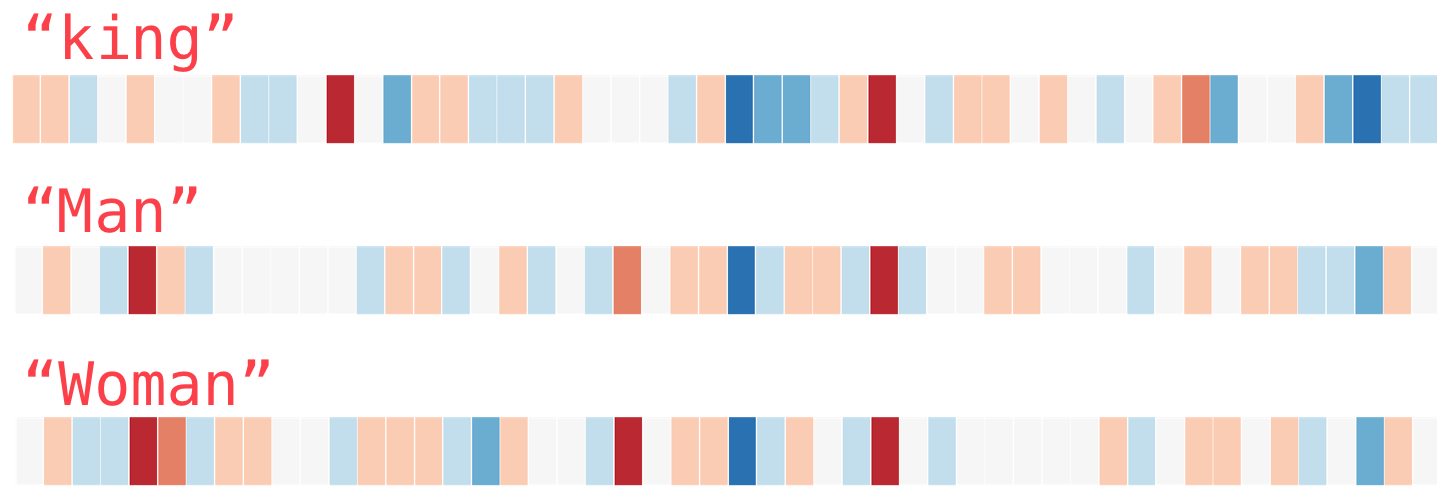
\includegraphics[width=.45\textwidth]{figures/king-man-woman-embedding.png}
  \caption{50-dimensional vector representation of \texttt{king} from Jay
    Alammar's \href{https://jalammar.github.io/illustrated-word2vec/}{The
    Illustrated Word2vec}. The embedding is a dense vector of elements in the
    reals. The deepest red denotes components with higher magnitude, those close
    to 1.6 and the coolest blue denotes values close to $-1.6$. One can see the
    similar components among all vectors (perhaps those encode a trait common to
    all entities, ``humanity'' in this case). One can observe the common
    components of `man' and `woman'}
\end{figure}

\subsection{Learning Semantic Representations}

One key property of word embedding models is that that they can be trained on
large corpora of unstructured text. This gives the key advantage that we can
retrain words representations as language continues to evolve. Two prominent
families of models  that exhibit semantic representations of words are
Continuous Bag-of-Words (CBOW) models and Skip-gram models.

In CBOW models, context is used to predict a target word
\citep{mikolov2013exploiting}. Formally, training example $(x,y)$ is constructed
by aggregating the representations of context words to form $x$, while the $y$.
In particular, this ``context'' is defined as the $k$-word window about the
target word $w_i$ in document $D$. If $k=2$, and the aggregation function is a
simple sum operation, then $x = \Sigma (w_{i-2}, w_{i-1}, w_{i+1}, w_{i+2})$ and
$y=w_i$. Then, $i$ is increased, advancing the sliding window throughout the
entire document, yielding further training examples. Emanating from this general
method, further variations exist to enhance performance including weighting words by distance to the target.

In Skip-Gram models, the training principle is flipped: a target word is used to
predict context words. The set of training examples would be $\{(w_i, w_{i-2}),
  (w_i, w_{i-1}), (w_i, w_{i+1}), (w_i, w_{i+2}) \}$
\citet{mikolov2013exploiting}. Then, in general, a dense neural network is
chosen to learn on these examples and a loss function encapulates the desire to
"maximize similarity between semantically similar words". A list of practial
differences between these two training schemes is presented in
\citet{mikolov2013exploiting}, but is elided here.

\begin{figure}
  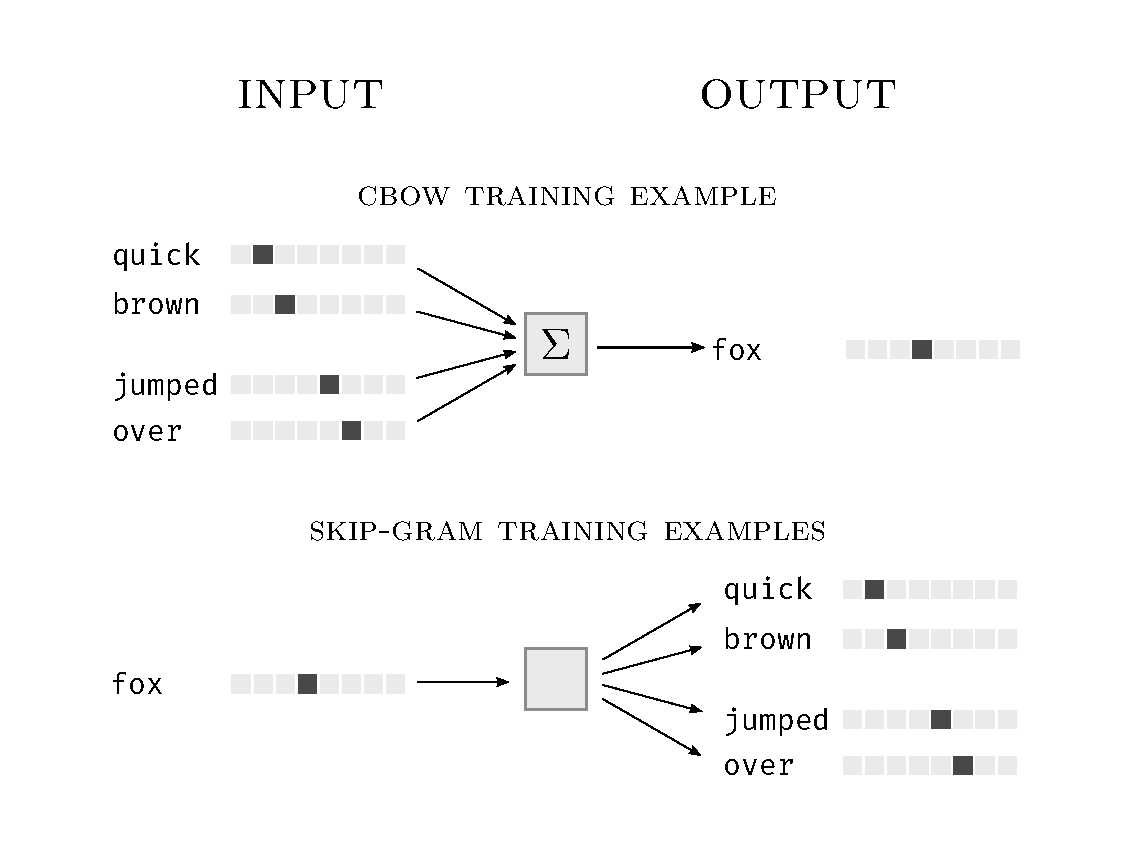
\includegraphics[width=0.5\textwidth]{figures/cbow-skipgram-train.pdf}
  \caption{This figure, inspired by one in  \citet{mikolov2013exploiting}
    illustrates the one-hot representations of words from the sentence ``The quick
    brown fox jumped over \dots'' being summed to form a CBOW training example,
    while multiple examples are formed with the skipgram model. The squares denote
    components in the one-hot vector, with black denoting the 1 and light grey
    denoting the 0 elements. \texttt{fox} $=w_4$ in this imaginary corpus, making
    \texttt{brown} $ = w_3$ and so on.}
\end{figure}



\subsection{Word Vector Arithmetic}

Let $T : V \to E$ denote the embedding operation of word $v$ from one-hot
encoded (large) vocabulary $V$ into embedding space $E$ with finite dimension
$\dim E$.  Then we can define arithmetic on these vector representations. Doing
so allows models to perform analogies.

$T(\text{king}) - T(\mathrm{man}) + T(\mathrm{woman})  \approx T(\mathrm{queen})$

And as a form of transfer learning, it acts as a way of imbuing models with
knowledge about syntactic and semantic relationships between words.

\section{Word Embedding Bias}

Reiterating $T : V \to E$ denotes the embedding operation of word $v$ from
vocabulary $V$ into embedding space $E$ with finite dimension $\dim E$, then we
produce the well-documented and infamous expression $ T(\text{computer
    programmer}) - T(\mathrm{man}) + T(\mathrm{woman})  \approx
  T(\mathrm{homemaker})$ from \cite{biased_analogy-1607-06520}, which clearly
exhibits the gender bias internalized by the learning algorithm that produced
it. Hereafter, I denote the vector representation of the word in upright
boldface.

The presence of these dubious associations is not unique to one architecture or
one configuration of hyper-parameters \cite{origins-1810-03611}. Thus, the
inclusion of a word embedding step may compromise the integrity of downstream
machine learning operations by injecting or accentuating this bias, making the
process unsuitable for a wide range of applications. In sensitive domains such
as granting loans, such model behavior may be illegal.

\section{Prior Work}

Many researchers have attempted to reduce bias in these embedding models, with
limited success. \citet{caliskan2017semantics}. These works can be partitioned
ito two categories. First, there are those that alter the training process in
some capacity. Then, there are those "post-processing" methods that alter vector
representations at the end of training. Two such works follow: they define bias
and attempt to minimize it without compromising performance on analogy tasks.

For example \citet{biased_analogy-1607-06520} formulate that the gender bias in a
non-gendered word can be quantified its scalar projection on the $\Vec{\textbf{he}} -
  \Vec{\textbf{she}}$ axis. They zero out the first principal component in the
gender direction.  \citet{lipstick-1903-03862} note that although the work was
"extensive, thoughtful, and rigorous", the approach of \citet{biased_analogy-1607-06520}
is inherently limited as the chosen definition of bias is hand-selected.

By contrast, \citet{zhao2018learning} also attempt to mitigate historical biases
in word embeddings, but they do so by altering the loss function of GloVe to
concentrate onto the last element the component of the embedding most correlated
with gender. Then, at inference time the last element of the embedding is
truncated away an thus discarded, "encouraging" the representations of
non-gendered words to be orthogonal to the gender direction.
\citet{lipstick-1903-03862} opine that this method carries the right intuition
-- the alterations the the model needs to happen at training time, but that the
execution has limited efficacy. In fact, ``indirect bias'' is still very obvious
even when ``direct bias'' is mitigated. They demonstrate that even simple models
can still learn the latent biases in the word embedding. This suggests that the
components of the vector that encode stereotypical notions of gender are
distributed as a linear combination of many components, even if they are
orthogonal to a primary ``gender dimension.''


The general critique of both methods is that the definition of bias relating to
distance to the gender direction \citet{lipstick-1903-03862} believe that the
correct method for removing gender bias, at a minimum, alters the training
process.

Furthermore, \citet{lipstick-1903-03862} remark that debiasing methods that
don't take the data into consideration merely "cover-up" the biases without
addressing the full associations themselves.

Historical Biases in Word Embedding models are pervasive:
The stereotypes reproduced by word embeddings are not just limited to gender,
but also extend to race and culture \citep{caliskan2017semantics}.

\section{WEAT: Operationalizing Bias}

\begin{figure}
  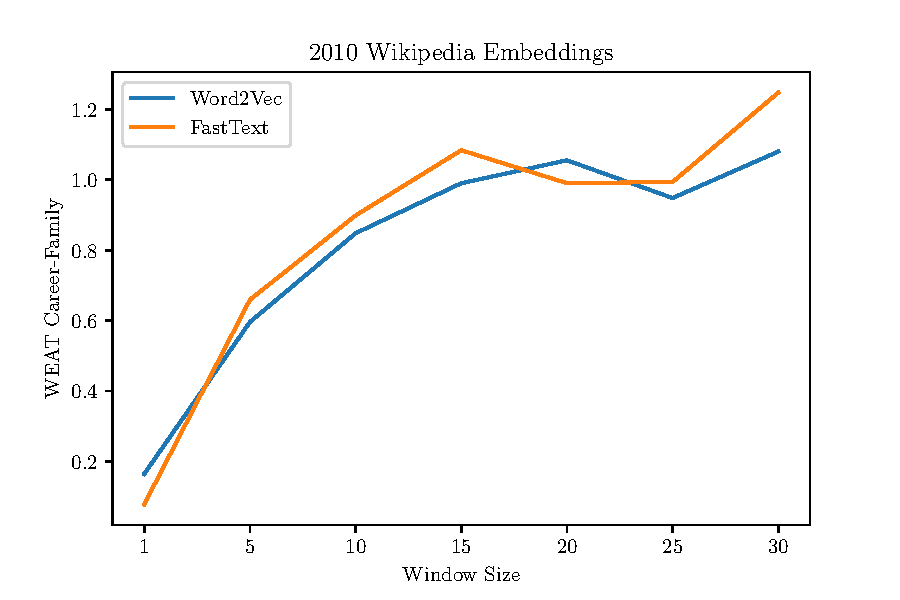
\includegraphics[width=.5\textwidth]{figures/car-fam_x_window_size_2010.pdf}
  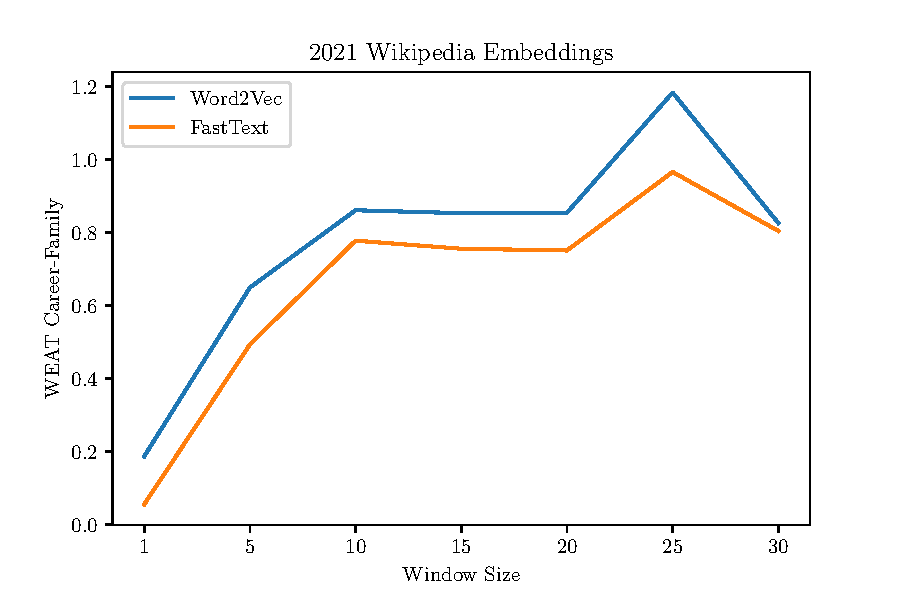
\includegraphics[width=.5\textwidth]{figures/car-fam_x_window_size_2021.pdf}
  \caption{This comparison between 2010 and 2021 Wikipedia Embeddings shows that
    they behave roughly the same: up to a point, larger window sizes produce
    embedding models with higher WEAT scores. It does not suggest that one year's
    data is any more biased than another's: learned gender bias in Wikipedia as
    measured by WEAT persists with time, however window size increases bias as measured by WEAT\label{weatxwindow}}
\end{figure}

As the desire to de-bias models gained traction, there was little consensus on
how to quantify bias, making it difficult to compare debiasing methods. Thus,
\citet{weat-1608-07187} developed the Word Embedding Association Test (WEAT) to
quantify how word embeddings capture empirical information about the world from
text corpora \citep[8]{weat-1608-07187}. WEAT score was modeled after the
Implicit Association Test (IAT) as a source of documented human biases
\citep[2]{weat-1608-07187}. Intuitively, WEAT can be understood as a
generalization of the use of word embedding models to perform analogies. They
first define  $s(w, A,B)= $
$$\\ \frac{ \text{mean}_{a \in A} \cos(\hat{w}, \hat{a} ) - \text{mean}_{b \in
      B} \cos(\hat{w}, \hat{b} ) } {\text{std}_{x\in A \cup B} \cos(\hat{w},
      \hat{x})}$$  and then $S(X,Y,A,B) = \sum_{x\in X} s(x, A, B) -  \sum_{y\in
      Y} s(y, A, B)$. That is, $S$ measures how close the associations between
      the target and attribute are. The more similar two sets of words are, the
      higher the WEAT score will be between them. The minimum WEAT score is -2
      and the maximum is 2. The higher WEAT score is, the higher the agreement
      between the embedding model and we WEAT axis.\footnote{To oversimplify, the higher
      the WEAT score is, the more it exhibits the particular bias along that
      axis.} WEAT has been performed along several axes with words corresponding
      to the IAT as mentioned prior. I use the Career-Family and Math-Art axes,
      but model behavior was consistent between them. It is useful to note that
      while the remainder of this work uses WEAT as a stand-in for historical
      bias, it is only one approach of many that quantifies these stereotypes.


\section{Experimental Setup}

To examine the behavior of historical biases in word embeddings over time, I
train GloVe and FastText word embedings using the Gensim library by
\citet{rehurek_lrec}.

How does model behavior influenced by context window size?  I declare window
sizes of $W = \{1,5,10,15,20, 25, 30\}$ about the target word. Narrower window
sizes usually encode syntactic relationships while longer sizes usually perform
better on semantic relationships such as relational analogies
\citet{clark2013handbook}.

I declare my architectures $A = \{\text{FastText},
  \text{Word2Vec} \}$; and corpora $C = \{\text{WikiSmall21} , \text{WikiSmall10}
  \}$ so named because they include only the first 330 MB of Wikipedia due to
computational constraints. For preprocessing, I used \citet{Wikiextractor2014}
to process the compressed archive of English Wikipedia. In all, I performed
experiments $W \times A \times C$ to examine the relationships between model
behaviors and window size, and how those behaviors change with time. Each year's
train-evaluate loop took about 90 minutes. Some portions are parallelized in
Gensim, while other portions run on a single thread.

\section{Evaluation}
\begin{figure}
  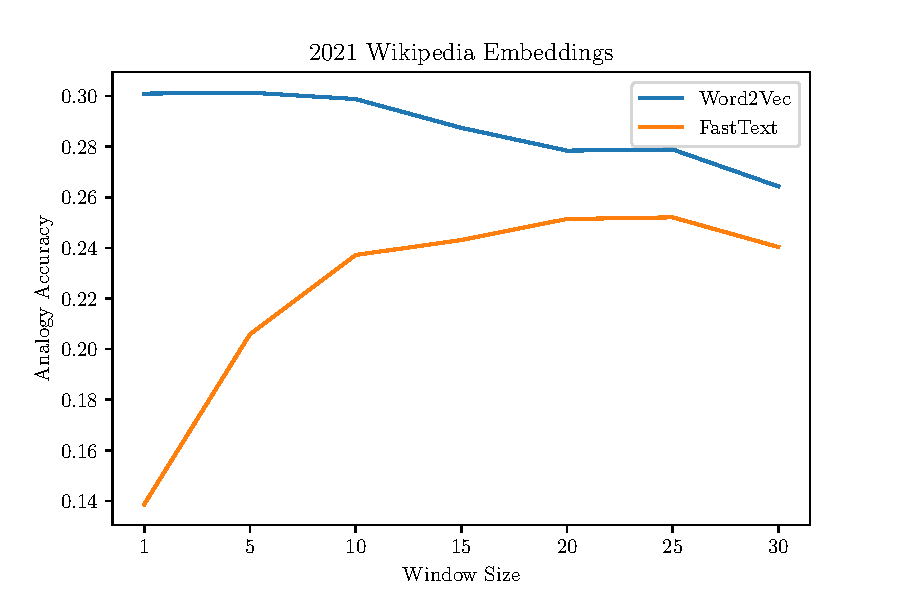
\includegraphics[width=.5\textwidth]{figures/analogy-avg_x_window_size_2021.pdf}
  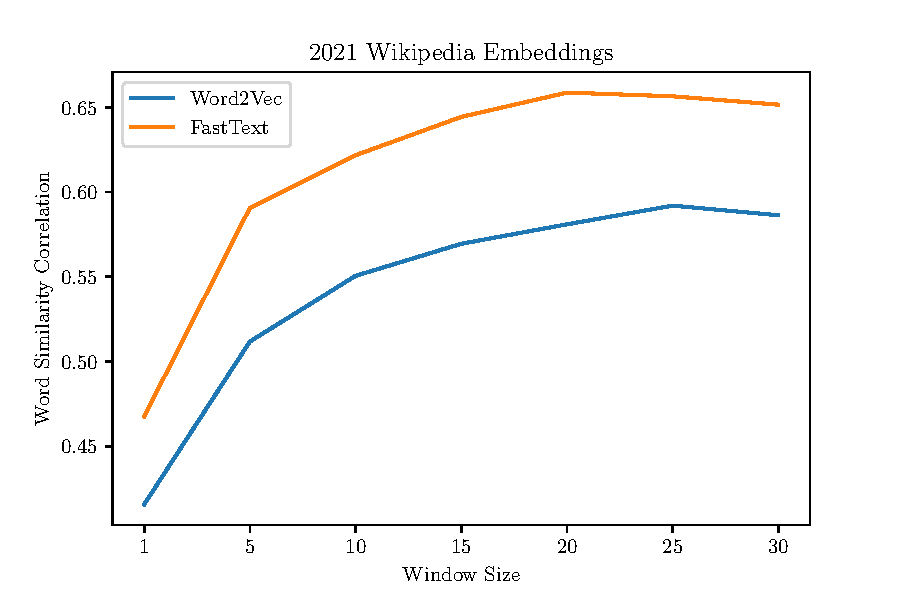
\includegraphics[width=.5\textwidth]{figures/wordsim_x_window-size_2021.pdf}
  \caption{The Analogy task (above) peaks early for Word2Vec, yielding a
    negative correlation with window size as more ``distracting'' words are
    introduced into the context window. FastText does not exhibit this property
    increasing before a plateau. Word Similarity (below) also responds positively
    with window size, also with diminishing returns as window sizes get large. \label{perf21}}
\end{figure}

Perhaps the most remarkable part of word embeddings trained in these ways is
that these vector representations can perform on tasks they were not trained
directly on, including word similarity. For example, using Pearson or Spearman
correlation, one can quantify how accurately the cosine of embedding
representations predicts degree of similarity WordSim353 from
\citep{agirre2009study}, with manually annotated word pairs quantifying
human-percieved ``similarity'' between the words.

For evaluation on analogies, one can use \citep{mikolov2013distributed} among
many choices. This has 19,544 instances and it is unbalanced, with 8,869
semantic and 10,675 syntactic questions, with betweeb 20-70 pairs per category.
Since country to capital relations comprise over 50 percent of all semantic
questions and in the 330 MB of training data, we can expect that there are many
missing words that count against the accuracy. There is an opportunity for
future work to compare different word sets.



\begin{figure}
  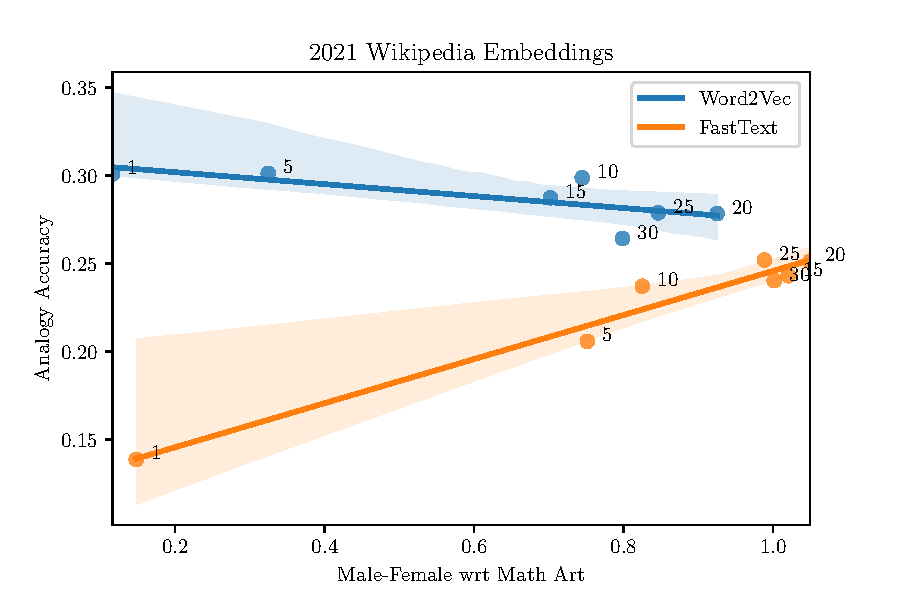
\includegraphics[width=.5\textwidth]{figures/analogy-avg_x_math-art_2021.pdf}
  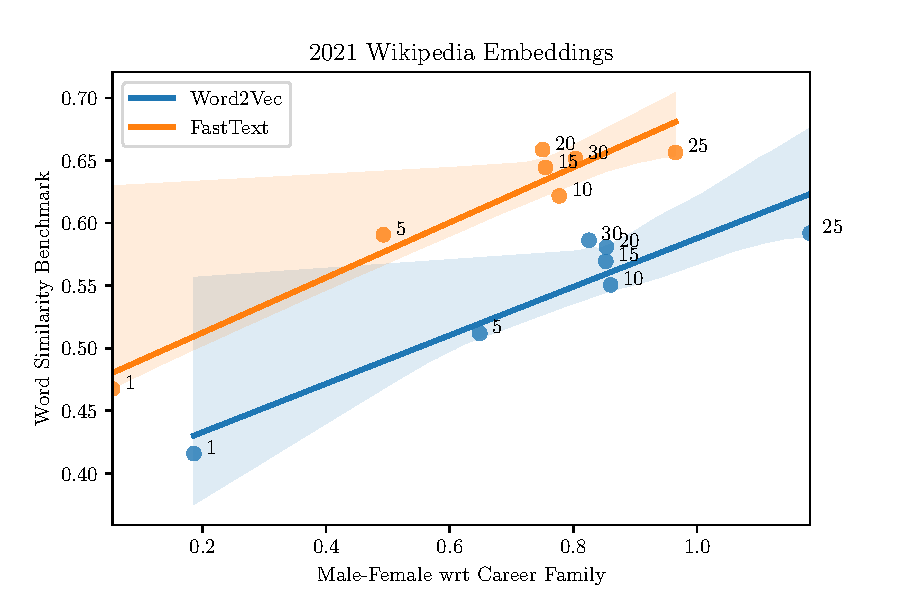
\includegraphics[width=.5\textwidth]{figures/car-fam_x_wordsim_2021.pdf}
  \caption{This is the scatter plot of Career-Family WEAT score against Analogy
    accuracy (above) and Word Similarity (below) this positive correlation
    suggests that models that have higer WEAT scores end to be the ones that
    perform better on convention benchmarks as well. \label{biasxperf}}
\end{figure}

\section{Results}

Figure~\ref{weatxwindow} suggests that as window size increases, so does WEAT
score. It suggests no substantive differences due to the passage of time in this
sample of the Wikipedia corpus. Figure~\ref{perf21} shows the result of window
size on conventional performance metrics. Figure~\ref{biasxperf} relates the
performance on conventional metrics to the Career-Family WEAT metric.

\section{Implications}

This reinforces the notion that word associations that reproduce historical
biases and stereotypes are learned the same way as factual word associations.
However, it is possible that there are analogies in the dataset that may
themselves exhibit stereotypes. In this case, a ``lesser-biased'' vector
representation may still exhibit a positive correlation as observed here. This
suggests the need to verify that the analogy set itself before proceeding
further with this claim.

\section{Limitations and Future Work}

\begin{enumerate}

  \item Chief on the list of limitations is the relatively small data size used and that
        training only occured for 1 epoch. Rather than the first 330 MB of data, future
        researchers can extend this to larger values keeping in mind the added training
        time.

  \item WEAT has come under question as a valid metric for quantifying bias. Future work
        might evaluate WEAT in conjunction with a variety of other methods of
        quantifying historical bias.

  \item There are many current attitudes discussing which domains are appropriate for
        debiasing, and whether some domains would benefit from ``faithful''
        representations of the world. Future work might choose to engage with this.

  \item There is work modeling analogy as probabilistic grammar and using statistical
        methods to learn analogies. Future work might compare these to word embeddings
        for these particular tasks.
  \item Sampling window sizes between 1, 5, and 10 might reveal trends that are
  not clearly visible with the current set of window sizes.
\end{enumerate}

\section{Acknowlegements}

Thank you Dr Anita Raja for helping me shape this research question and for
extensive feedback at every step of this process. Furthermore, thank you Dr
Sarah Ita Levitan for providing insight into practial considerations when
incorporating a word embedding step and associated discussion and sparking my
original interest in the topic.

\bibliographystyle{acl_natbib}
\bibliography{arr}

%\appendix



\end{document}
